\documentclass[12pt]{article}
\usepackage{hyperref}
\usepackage{mathtools}
\usepackage{tabto}
\usepackage{pgfplots}
\begin{document}
	
	\title{\Huge \textbf{Esercizi}}
	\date{\today}
	\maketitle	
	\pagenumbering{gobble}		
		
	\section*{3 Ottobre}
			\textbf{\large 1} \\
			\textit{Quante sono le sequenze date da due difre decimali?} \\\\
			\textbf{Soluzione} \\
			$\{00,01,02,...,09,10,11,...,99\}$ La somma di tali sequenze \`e $100$. \\\\
			\textbf{\large 2} \\
			\textit{Un cammino reticolare è un percorso sul piano cartesiano che 			effettua passi di lunghezza uno verso destra o verso l’alto. Quanti 				sono i cammini reticolari da $(0,0)$ a $(2,2)$?} \\\\
			\textbf{Soluzione} \\
			1 percorso: fissiamo una sola direzione di partenza e muoviamoci verso questa finch\`e non sar\`a necessario cambiarla.
			$n-1$ percorsi: partendo dall'ultimo movimento del percorso precedente modifichiamo il pi\'u vicino in modo tale da creare un percorso diverso da quello precedente. \\ 
			Percorsi totali: $6$. \\\\			
			\textbf{\large 3} \\
			\textit{Mostrare che esiste una corrispondenza biunivoca tra i cammini reticolari (vedi esercizio precedente per la definizione) da $(0,0)$ a $(3,2)$ e i sottoinsiemi di $\{1,2,3,4,5\}$ di cardinalit\`a $2$.}	\\\\
			\textbf{Soluzione} \\
			Notando che il numero totale di movimenti per arrivare a $(3,2)$ è pari a 5 (elementi dell'insieme) e che gli spostamenti verso l'alto sono necessariamente 2 (elementi del sottoinsieme di cardinalit\`a 2), possiamo pensare al numero di ogni sottoinsieme come il numero del movimento in cui ci spostiamo verso l'alto:\\
			
			\begin{center}
           		$\{1,2\} \rightarrow$ primo e secondo movimento verso l'alto\\
				$\vdotswithin{}$\\
            	$\{1,5\} \rightarrow$ primo e quinto movimento "	"\\
            	$\{2,3\} \rightarrow$ secondo e terzo movimento "	"\\
				$\vdotswithin{}$\\
            	$\{4,5\} \rightarrow$ quarto e quinto movimento "	"\\
            \end{center}
			\textbf{\large 4} \\
			\textit{Esibire una corrispondenza biunivoca tra  gli intervalli aperti reali $(0,1)$ e $(5,10)$.} \\\\
			\textbf{Soluzione} \\		
			$f: ]0,1[ \longrightarrow ]5,10[$	\\		
			$f(x)=5x+5$ \\\\
			$f$ \`e iniettiva? \\
			$5x+5=5x'+5$ \\
			$\rightarrow x=x'$\\
			$f$ \`e suriettiva? \\
			$y \in (5,10)$ \\
			$y=5x+5 \longleftrightarrow x= \frac{y-5}{5}$ \\\\

            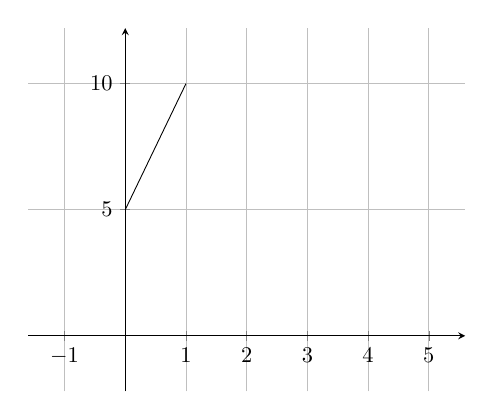
\begin{tikzpicture}[scale=0.81, trim axis right]
            	\begin{axis}[grid=both,xmin=-1,xmax=5,ymin=-1,ymax=11,axis lines=middle,enlargelimits]
            	\addplot[domain=0:1] {5*x+5};            
            	\end{axis}            
            \end{tikzpicture} 
            \\\\
            \textbf{\large 5} \\
			\textit{Mostrare che i sottoinsiemi di cardinalit\`a pari di un insieme con 10 elementi sono tanti quanti quelli di cardinalit\`a dispari (sugg.: aggiungere o togliere un elemento da un sottoinsieme cambia la parità della sua cardinalit\`a).} \\\\
			\textbf{Soluzione} \\
			Per Def. le combinazioni di lunghezza $k$ in $A$, dove $|A|=n$ sono i sottoinsiemi di $A$ con $k$ elementi:
			\[
				\binom{n}{k} = \frac{n!}{k!(n-k)!}
			\]
			Binomio di Newton: \\
			\[
				(a+b)^n = \sum_{k=0}^{n} \binom{n}{k}a^k b^{n-k}
			\]
			Se $a=1,b=-1$ :
			\[
				0=(1-1)^n = \sum_{k=0}^{n} \binom{n}{k}1^k -1^{n-k}
			\]
			$n=10$ :
			\[
				\binom{10}{0} - \binom{10}{1} + \binom{10}{2} - \cdots + \binom{10}{10} =0 
			\]
    		\[
				\binom{10}{0} + \binom{10}{2} + \binom{10}{4} + \cdots + \binom{10}{10} = \binom{10}{1} + \binom{10}{3} + \binom{10}{5} +  \binom{10}{7} + \binom{10}{9}
			\]
			\\
			$\Longrightarrow$ I sottoinsiemi di cardinalit\`a pari sono tanti quelli di cardinalit\`a dispari.
			\\\\
			\textbf{\large 6} \\
			\textit{Quante sono le sequenze binarie lunghe 5,6,7 in cui non compaiono mai due 1
consecutivi? (Sugg. Iniziare con sequenze pi\`u corte e cercare di capire una
regola ricorsiva)} \\\\
			\textbf{Soluzione} \\
			Procedimento: partendo dalla sequenza $0$ ed $1$ dove $n=1$ costruiamo le successive $n=2\ldots$ aggiungendo uno 0 per ogni sequenza lunga $n-1$ e un $1$ alle sequenze che iniziano con uno $0$.
			\begin{itemize}
				\item $n=1 \rightarrow 0,1$ 
				\item $n=2 \rightarrow 00,01,10$
				\item $n=3 \rightarrow  000,001,010,100,101$
			\end{itemize}
			$\>$ $\>$ $\-$ \vdots \\\\
			Le sequenze lunghe $n$ che iniziano con $0$ sono tante quante quelle lunghe $n-1$, quelle che iniziano con $n-1$ sono tante quante quelle lunghe $n-2$.\\ \textit{Numeri di Fibonacci}	:\\\\		
			\[
				F(n) = \begin{cases} F(n-1)+F(n-2) & \mbox{if } n\geq\mbox{3} \\ 
				3 & \mbox{if } n=\mbox{2} \\
				2 & \mbox{if } n=\mbox{1}
				\end{cases}
			\]
			\\
			$F(5)=F(4)-F(3)=[F(3)+F(2)]-[(F(2)+F(1)] = 13 \\
			F(6)=21, F(7)=55$ 
			\\\\
			\textbf{7} \\
			\textit{Quante sono le sequenze binarie lunghe 5,6,7 in cui non compaiono mai tre 1
consecutivi? (Sugg. Iniziare con sequenze più corte e cercare di capire una
regola ricorsiva)} \\\\
			\textbf{Soluzione} \\
			Simile all'esercizio precedente: \\
			\begin{itemize}
				\item $n=1 \rightarrow 0,1$ 
				\item $n=2 \rightarrow 00,01,10,11$
				\item $n=3 \rightarrow 000, 001, 010, 011, 100, 101, 110$
			\end{itemize}
			$\>$ $\>$ $\-$ \vdots \\\\
			\[
				G(n) = \begin{cases} G(n-1)+G(n-2)+G(n-3) & \mbox{if } n\geq\mbox{4} \\ 
				7 & \mbox{if } n=\mbox{3} \\
				4 & \mbox{if } n=\mbox{2} \\
				2 & \mbox{if } n=\mbox{1}
				\end{cases}
			\]
			\\
			$G(5)=24, G(6)=44, G(7)=81$ \\\\ 
			
			

			
	            
\end{document}
